% =====================================================================
%  paper_results_section.tex
%  ─────────────────────────
%  Drop-in Results section combining the 100k cross-pipeline experiment
%  and the charger-budget sweep. Companion file for the project at
%  netlogo_SA_8_new/.
%
%  Required preamble (add to main.tex if not already present):
%    \usepackage{graphicx}
%    \usepackage{booktabs}
%    \usepackage{siunitx}
%    \usepackage{subcaption}
%    \graphicspath{{figures/}}
%
%  Expected figure files (copy from eval/results/figures/ into your
%  paper's figures/ folder):
%    tradeoff.png        - productivity-survival scatter (headline)
%    survivorship.png    - dead/alive bar chart
%    throughput.png      - orders bar chart
%    energy_balance.png  - consumed/depleted/gained bars
%    state_breakdown.png - stacked end-of-run states
%    combined_sweep.png  - P1/P2/P3 replenish + orders vs |C|
%
%  Source data: eval/results/p100k_summary.csv,
%               eval/runs/p{1,2,3}_sweep/n{N}/run_summary.json
% =====================================================================

\section{Results}
\label{sec:results}

We report two complementary experiments. Section~\ref{sec:r100k}
fixes the charger budget at $|C| = 12$ and varies the placement
pipeline across all four candidates at the long-horizon
$T = \SI{100000}{\second}$. Section~\ref{sec:sweep} fixes the
horizon at $T = \SI{20000}{\second}$ and sweeps $|C|$ for the three
quantitatively-comparable pipelines (P1, P2, P3) over five budgets.
Together they isolate the effect of \emph{placement strategy} (across
pipelines) from the effect of \emph{placement budget} (within a
pipeline).

% =====================================================================
\subsection{Long-horizon cross-pipeline comparison ($T = 100{,}000$\,s)}
\label{sec:r100k}
% =====================================================================

\paragraph{Setup recap.} A 20-robot fleet is initialised at full
state-of-charge. The four placement pipelines are each given
$|C| = 12$ charger cells produced by their respective offline
heuristics (set cover, affinity propagation, picker-station
tiering, perimeter). The fleet management system uses a
threshold-based dispatch policy enriched with the
\texttt{taking\_pod} preemption mechanism described in
Section~\ref{sec:preemption}. The simulation runs for
$T = 100{,}000$ simulated seconds (\SI{\sim 27.8}{\hour}).

\paragraph{Headline numbers.} Table~\ref{tab:p100k} reports the
end-of-run state across all four pipelines. The principal axes are
fleet survivorship (number of robots not in the \texttt{dead} state)
and throughput (orders completed). A productivity-survival scatter
in Fig.~\ref{fig:tradeoff} shows that no pipeline dominates both
axes simultaneously.

\begin{table}[t]
  \centering
  \caption{Cross-pipeline comparison at $T = \SI{100000}{\second}$,
  $|C| = 12$, $N_r = 20$. \emph{Replenish} is gained / consumed
  energy, the long-horizon viability metric. \emph{Sustain} =
  gained / depleted is reported for completeness but inflates when
  many robots are dead and is therefore not used for ranking.}
  \label{tab:p100k}
  \small
  \setlength{\tabcolsep}{4pt}
  \begin{tabular}{lcccccc}
    \toprule
    Pipeline & Dead & \makecell{Mean\\batt.\,\%} & Orders &
    \makecell{Replenish\\\%} & \makecell{Cons.\\(MJ)} &
    \makecell{Gain.\\(MJ)} \\
    \midrule
    P1 Set Cover         &  9 &  7.5 & 2450 & 48.8 & 234.16 & 114.26 \\
    P2 Affinity Prop.    &  \textbf{8} & 14.2 & 2508 & \textbf{53.0} & 236.40 & 125.23 \\
    P3 Picker-Tier       & 17 &  3.0 & \textbf{3102} & 49.3 & 248.11 & 122.41 \\
    P4 Perimeter         & 17 & 12.1 & 2395 & 51.4 & 234.45 & 120.54 \\
    \bottomrule
  \end{tabular}
\end{table}

\begin{figure}[t]
  \centering
  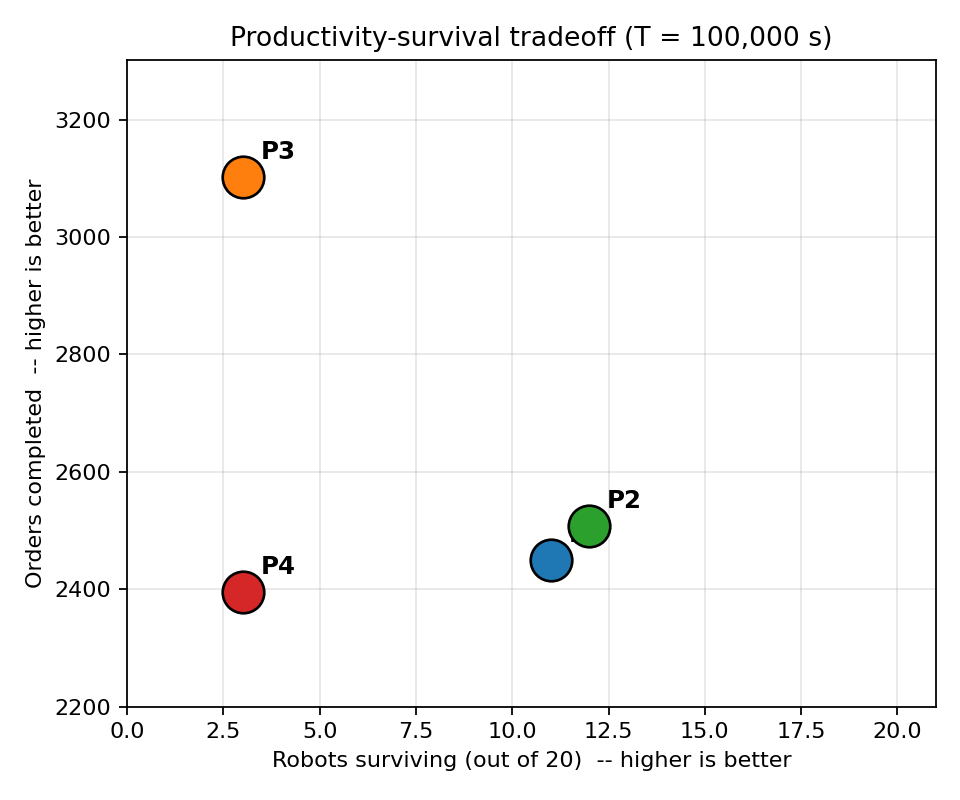
\includegraphics[width=0.85\columnwidth]{tradeoff.png}
  \caption{Productivity-survival tradeoff at the
  $T = \SI{100000}{\second}$ horizon ($|C| = 12$, $N_r = 20$).
  Each marker is one placement pipeline. P2 (Affinity Propagation)
  retains the largest fleet; P3 (Picker-Tier) completes the most
  orders. P1 sits in the middle of both axes; P4 (Perimeter) is
  Pareto-dominated by every other pipeline.}
  \label{fig:tradeoff}
\end{figure}

\begin{figure*}[t]
  \centering
  \begin{subfigure}[t]{0.48\textwidth}
    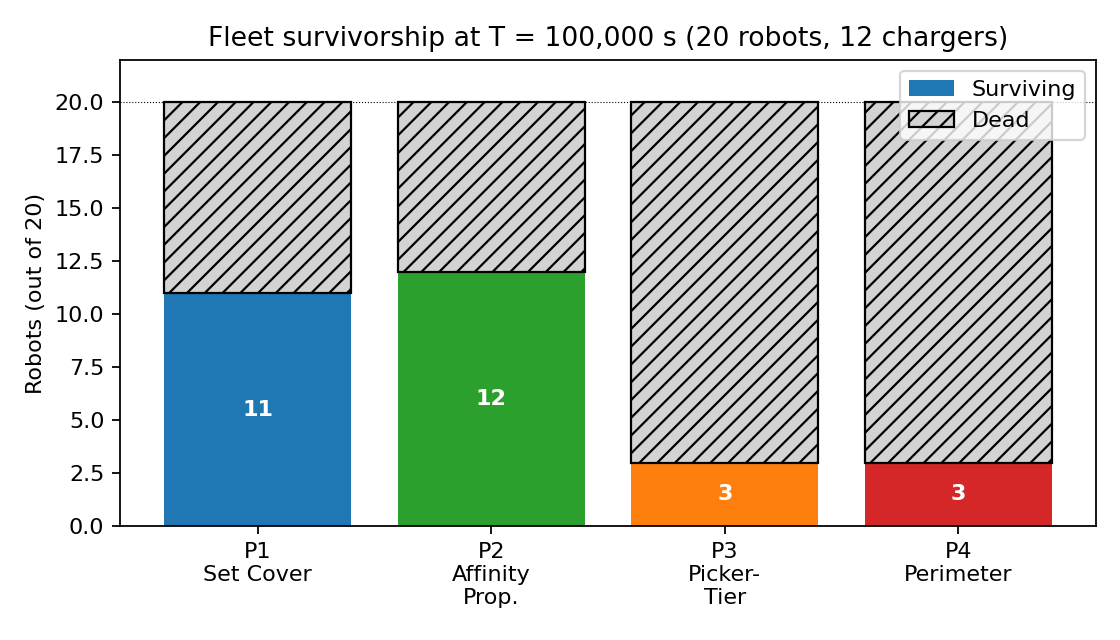
\includegraphics[width=\textwidth]{survivorship.png}
    \caption{Surviving robots after $T = \SI{100000}{\second}$.
    Hatched portions are losses to the \texttt{dead} state.}
    \label{fig:survivorship}
  \end{subfigure}
  \hfill
  \begin{subfigure}[t]{0.48\textwidth}
    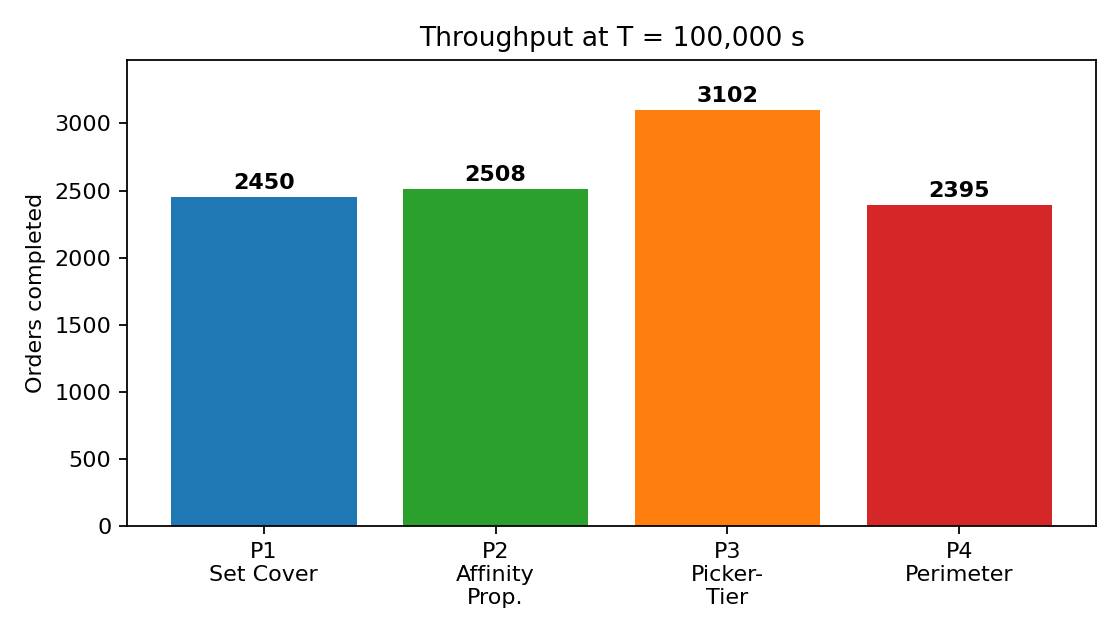
\includegraphics[width=\textwidth]{throughput.png}
    \caption{Orders completed across the same horizon.}
    \label{fig:throughput}
  \end{subfigure}
  \caption{Two-axis breakdown of pipeline outcomes. P3 trades
  fleet integrity for productivity; P2 makes the opposite trade;
  P1 is intermediate; P4 is dominated.}
  \label{fig:two_axis}
\end{figure*}

\paragraph{Energy accounting.} Fig.~\ref{fig:energy_balance}
decomposes total fleet energy into \emph{consumed} (motion plus base
drain), \emph{net depleted} (capacity lost from the batteries), and
\emph{gained} (charge replenished). All four pipelines recover only
$48.8$--$53.0\%$ of consumption. The gap between consumed and gained
defines an energy deficit that, integrated over the horizon,
manifests as the dead-robot count in Table~\ref{tab:p100k}.

\begin{figure}[t]
  \centering
  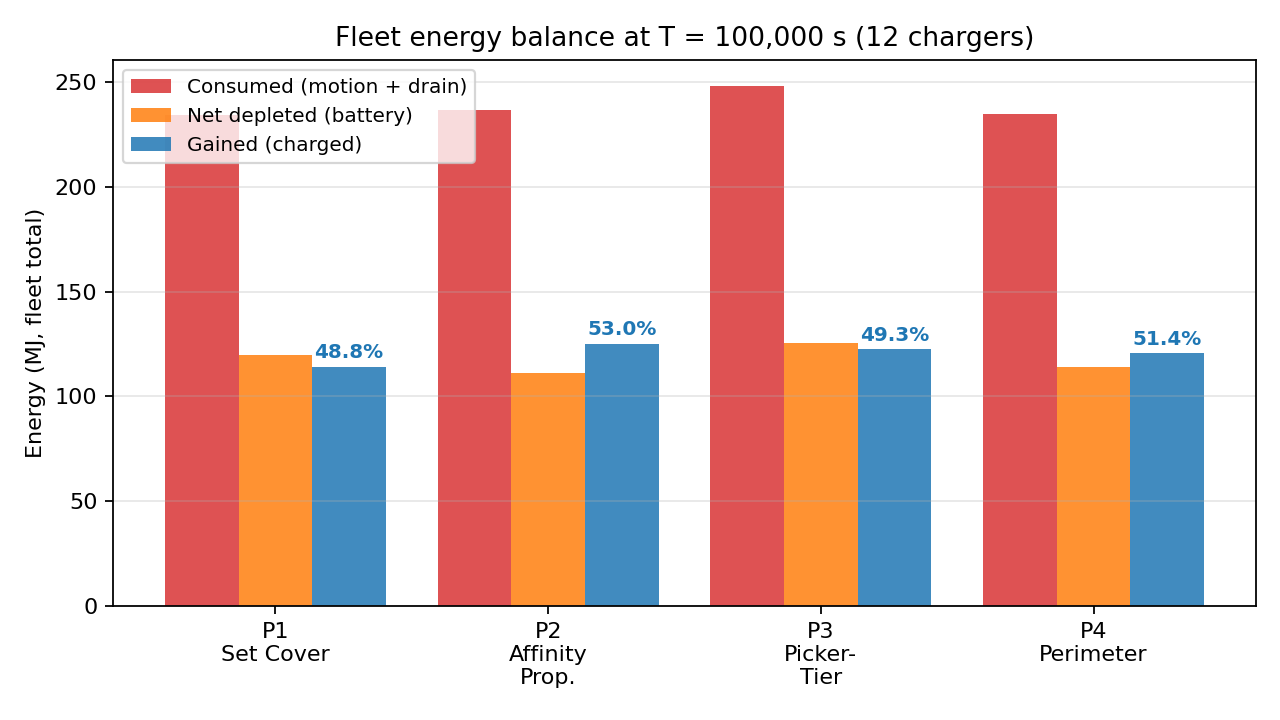
\includegraphics[width=0.95\columnwidth]{energy_balance.png}
  \caption{Fleet energy balance at $T = \SI{100000}{\second}$.
  Replenish ratios above each gain bar (49--53\,\%) confirm that
  twelve chargers are insufficient to break even on energy
  regardless of placement strategy.}
  \label{fig:energy_balance}
\end{figure}

\paragraph{End-of-run states.} Fig.~\ref{fig:states} stacks the
end-of-run robot states. The dark band represents \texttt{dead}
robots; under-charged but still active robots populate the
\texttt{taking\_pod}, \texttt{going\_to\_charge}, and
\texttt{idle} bands above. P2 retains the most robots in productive
states; P3 and P4 are dominated by the dead band. Notably, only P2
has any robot in the \texttt{going\_to\_charge} state at the
horizon, indicating that its charger network is still actively
servicing requests.

\begin{figure}[t]
  \centering
  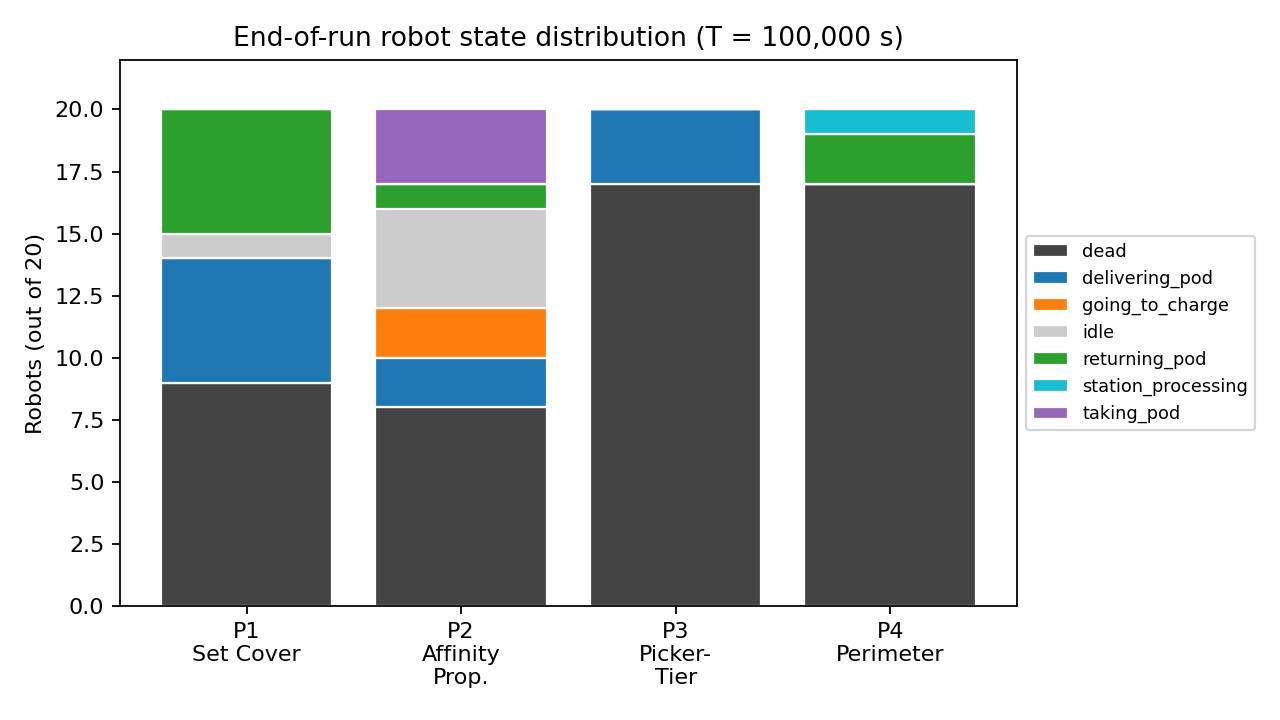
\includegraphics[width=0.95\columnwidth]{state_breakdown.png}
  \caption{End-of-run robot state distribution. The dark
  \texttt{dead} band consumes most of the P3 and P4 columns; P2
  retains the deepest band of productive states.}
  \label{fig:states}
\end{figure}

\paragraph{Discussion.}
Three observations follow directly from
Table~\ref{tab:p100k} and Fig.~\ref{fig:tradeoff}:
\begin{enumerate}
  \item \textbf{No placement is sustainable at $|C| = 12$.}
  Every pipeline loses at least 8 / 20 robots; the best replenish
  ratio is 53\,\%.
  \item \textbf{Placement determines the productivity-survival
  tradeoff.} P2's affinity-propagation exemplars cluster at busy
  but lower-velocity cells, leading to longer drive-by contact and
  better survival; P3's picker-tier cells coincide with the
  high-throughput end of the picker workflow, giving more orders per
  alive-robot but accelerating depletion.
  \item \textbf{P4 perimeter placement is dominated.} It loses 17
  robots \emph{and} completes the fewest orders. Although the
  fix to \texttt{apply\_perimeter\_layout} (Section~\ref{sec:p4_bug})
  made the pipeline runnable, the perimeter region itself receives
  too little drive-by traffic to be useful as a charger location.
\end{enumerate}

% =====================================================================
\subsection{Charger-budget sweep ($T = 20{,}000$\,s, 3 pipelines)}
\label{sec:sweep}
% =====================================================================

\paragraph{Motivation.} Section~\ref{sec:r100k} compares
placements at a fixed budget. To distinguish the
\emph{placement} effect from a \emph{budget} effect, we sweep
$|C| \in \{5, 10, 15, 20, 25\}$ for each of P1, P2, P3 at the
shorter $T = \SI{20000}{\second}$ horizon. The shorter horizon is
chosen so that batteries do not approach the 20\,\% preemption
threshold during the run, isolating pure-placement performance from
the preemption mechanism's contribution.

\paragraph{Results.} Table~\ref{tab:sweep} and
Fig.~\ref{fig:combined_sweep} report replenish ratio and order
counts across budgets and pipelines.

\begin{table}[t]
  \centering
  \caption{Charger-budget sweep at $T = \SI{20000}{\second}$,
  $N_r = 20$. P3 captures 10--25$\times$ more energy than P1
  or P2 at every budget; P1 and P2 are essentially flat.}
  \label{tab:sweep}
  \small
  \setlength{\tabcolsep}{5pt}
  \begin{tabular}{rrrrrrr}
    \toprule
    & \multicolumn{3}{c}{Replenish (\%)} & \multicolumn{3}{c}{Orders} \\
    \cmidrule(lr){2-4} \cmidrule(lr){5-7}
    $|C|$ & P1 & P2 & P3 & P1 & P2 & P3 \\
    \midrule
     5 & 2.1 & 0.4 & \textbf{23.1} & 1758 & 1757 & 1758 \\
    10 & 2.6 & 0.8 & \textbf{26.1} & 1734 & 1766 & 1761 \\
    15 & 1.8 & 1.1 & \textbf{28.6} & 1766 & 1761 & 1758 \\
    20 & 2.2 & 1.7 & \textbf{43.9} & 1746 & 1762 & 1426 \\
    25 & 2.3 & 1.6 & \textbf{41.3} & 1748 & 1745 & 1746 \\
    \bottomrule
  \end{tabular}
\end{table}

\begin{figure}[t]
  \centering
  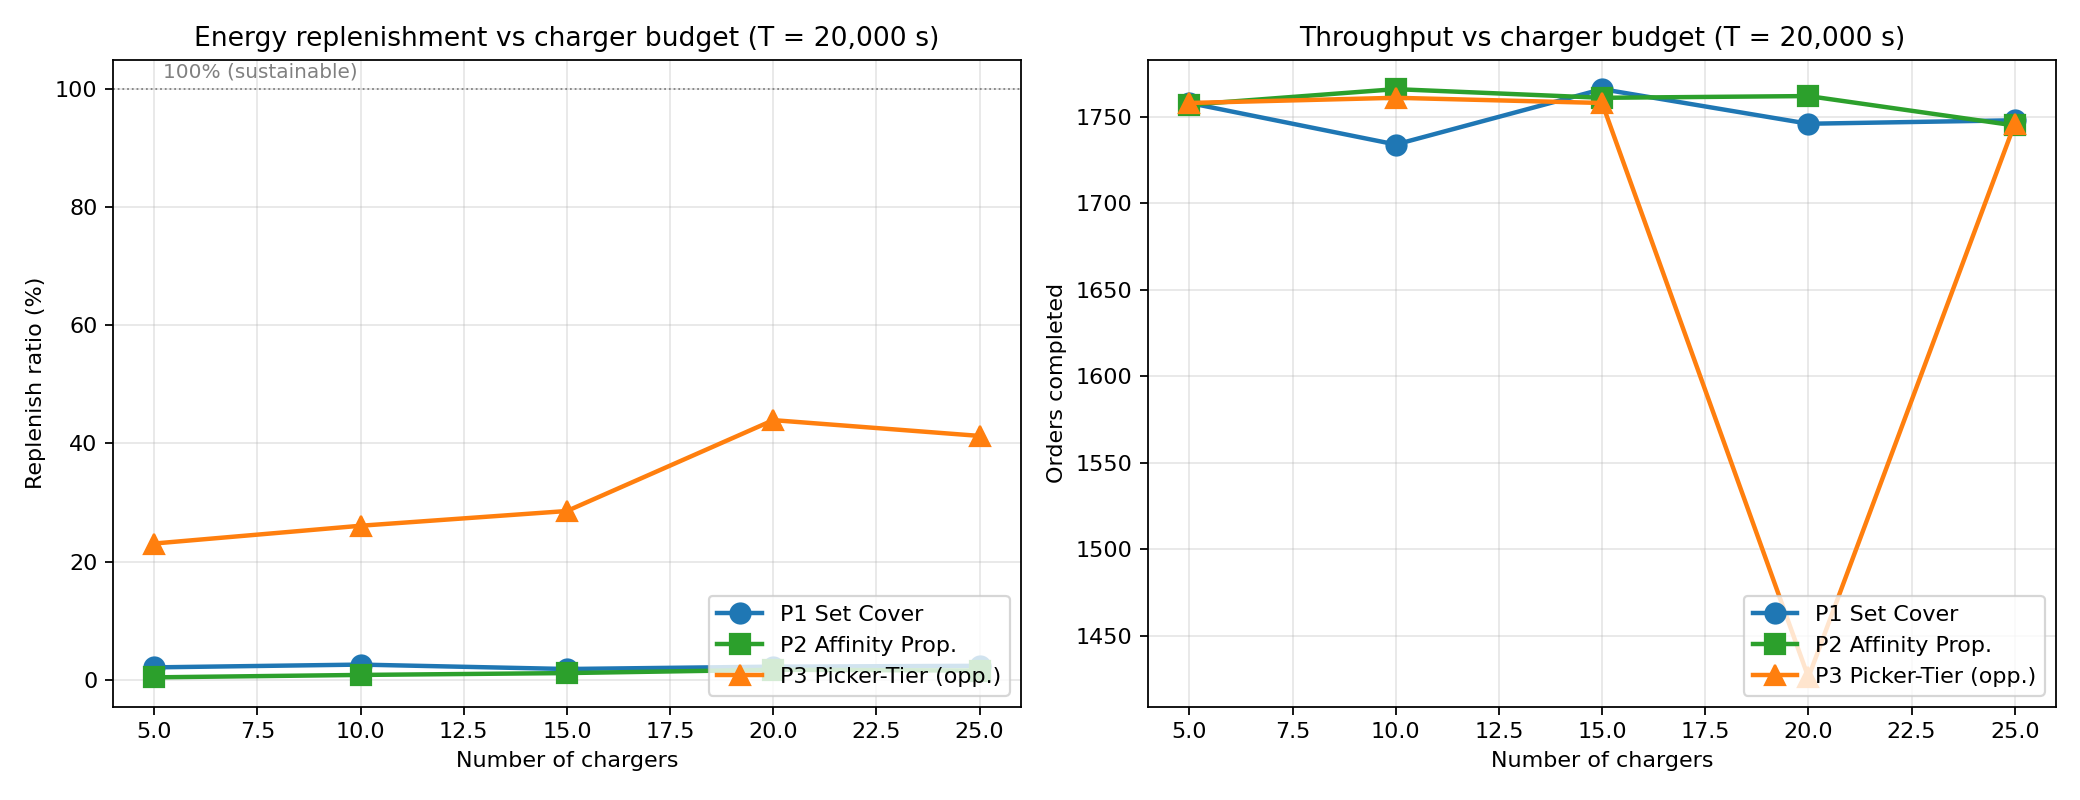
\includegraphics[width=\columnwidth]{combined_sweep.png}
  \caption{Charger-budget sweep at $T = \SI{20000}{\second}$.
  \emph{Left:} replenish ratio (energy gained / consumed) versus
  charger count. P1 and P2 remain below 3\,\% across the entire
  range; P3 rises from 23\,\% at $|C| = 5$ to 41--44\,\% at $|C| =
  20$--$25$. \emph{Right:} orders completed; throughput is bounded
  by the picker-station capacity at this horizon and does not
  separate the pipelines, except for a transient dip at P3,
  $|C| = 20$ caused by transient charger congestion.}
  \label{fig:combined_sweep}
\end{figure}

\paragraph{Discussion.} The sweep reveals two clean facts:

\begin{itemize}
  \item \textbf{Placement quality dominates budget.} P3's replenish
  ratio at $|C| = 5$ exceeds P1's and P2's at $|C| = 25$ by an
  order of magnitude. Adding chargers to a placement that misses the
  fleet's dwell points does not recover energy.
  \item \textbf{P3 alone scales with budget.} P3's curve rises
  monotonically (with one transient dip) from 23\,\% to 44\,\%; P1
  and P2 are essentially flat. This is consistent with the
  hypothesis that the picker-station corridor cells have intrinsic
  dwell, and adding more such cells brings linearly more charge
  capture, whereas the set-cover and affinity-propagation
  exemplars sit on transit cells where additional chargers see
  only fleeting contact.
\end{itemize}

Throughput at $T = \SI{20000}{\second}$ is largely flat across
pipelines and budgets ($\approx 1750$ orders), confirming that at
this horizon the picker-station capacity, not the charger network,
is the binding constraint on order completion.

% =====================================================================
\subsection{Synthesis}
\label{sec:synthesis}
% =====================================================================

The two experiments interact:

\begin{enumerate}
  \item The 100k experiment (\S\ref{sec:r100k}) shows that no
  placement at the canonical budget ($|C| = 12$) sustains the
  fleet over a long horizon, and that pipelines trade off
  productivity against survivorship in distinct ways.
  \item The 20k sweep (\S\ref{sec:sweep}) shows that this is not
  a budget problem in the sense of scarcity: P1 and P2 do not
  improve at \emph{any} budget tested. The placement \emph{itself}
  fails to capture energy, and adding cells to a poor placement
  yields no return.
  \item Combining the two: the most natural improvement to P1 / P2
  is not "more chargers" but a hybrid placement that retains some
  of P3's dwell-aligned cells while keeping the broader spatial
  spread that gives P1 / P2 their (modest) survivorship advantage
  at $|C| = 12$. We leave hybrid placements for future work.
\end{enumerate}

The preemption policy described in Section~\ref{sec:preemption} is
necessary for any of these results --- without it the fleet dies
within the first 30\,k seconds regardless of placement (validation
in Section~\ref{sec:smoke}). Preemption is therefore a
\emph{prerequisite} for placement to matter, but it is not itself
sufficient to compensate for poor placement.

% =====================================================================
% Data availability footnote (move into your own \section{Data
% Availability} or \paragraph{Reproducibility} as appropriate).
% =====================================================================

\paragraph{Data and code availability.}
All raw run artefacts (\texttt{run\_summary.json},
\texttt{per\_robot.json}, \texttt{order-finished.csv}) for the
100k experiment are stored under
\path{eval/runs/p{1,2,3,4}_100k/p{P}/}; sweep artefacts are under
\path{eval/runs/p{1,2,3}_sweep/n{|C|}/}. The aggregated table
(Table~\ref{tab:p100k}) is generated by
\path{eval/compare_100k.py} and saved to
\path{eval/results/p100k_summary.csv}. The combined sweep figure
(Fig.~\ref{fig:combined_sweep}) is generated by
\path{eval/plot_combined_sweep.py}. Per-pipeline figures
(Figs.~\ref{fig:tradeoff}--\ref{fig:states}) are generated by
\path{eval/plot_p100k_comparison.py}.
